\documentclass[10pt,a4paper]{article}
\usepackage{fontspec,polyglossia}
\setmainlanguage{russian}
\setmainfont{Times New Roman}
\usepackage{amsmath,amssymb,booktabs,tabularx,graphicx}
\usepackage[margin=17mm]{geometry}
\usepackage[hidelinks]{hyperref}
\usepackage{titlesec}
\titleformat{\section}{\large\bfseries}{}{0pt}{}
\titlespacing*{\section}{0pt}{8pt}{4pt}
\setlength{\parindent}{0pt}
\setlength{\parskip}{4pt}
\setlength{\emergencystretch}{3em}
\begin{document}
{\Large\bfseries MG при потере информации в текстовом VAE: 10 инициализаций}\par\medskip

Расширение серии, 29 сентября 2026. Пилот seed 0; подтверждение seeds 1--9, включая семь добавленных запусков 3--9. Все пары и исходные логи сохранены.

\textbf{Основной результат:} независимое событие подтверждено в 9/9 подтверждающих запусков. MG на фиксированной ошибке восстановления показал более сильное снижение, чем контроль, в 9/9, в том числе в 7/7 добавленных запусков. Медиана парного отношения $q=0,517$; диапазон 0,430--0,599. Пилот исключён из этих чисел. Неудачные seed по основному критерию: нет.

\section*{1. Что учится и что считаем упрощением}

Текстовый VAE восстанавливает предложения: encoder преобразует целое предложение в распределение скрытого кода, decoder предсказывает слова по предыдущим словам и этому коду. Проверяем ослабление роли кода при обучении. Если в коде становится мало информации о предложении, а его подмена почти не меняет предсказания, эта часть модели фактически перестаёт решать исходную задачу представления текста. Это операционное упрощение латентного механизма, не доказательство уменьшения размерности всей системы.

\textbf{Данные и модель.} Penn Treebank, фиксированные 6000 обучающих и 256 проверочных предложений, длина 8--24 слова плюс EOS. Словарь 2000 токенов строится по обучающей части; в проверке около 18,4\% токенов представлены UNK. Embedding 48, encoder GRU 64, Gaussian latent 16, decoder GRU 64; 276016 параметров. Код подаётся в начальное состояние decoder и на каждом шаге. Teacher forcing, без dropout. Adam: learning rate 0,001, batch 32, clipping нормы градиента 5.

Loss --- сумма NLL слов предложения плюс $\beta\,\mathrm{KL}(q(z\mid x)\Vert\mathcal N(0,I))$, затем среднее по батчу. После общих 1024 обновлений при $\beta=0{,}01$ создаются две ветви: \textbf{base} сохраняет коэффициент, \textbf{regularized} повышает его до 1. Обе обучаются до 3072 шагов. Веса, Adam и генератор батчей/латентного шума совпадают при развилке. Learning rate и размер кода не меняются; координаты вручную не выключаются.

\section*{2. Независимое подтверждение и наблюдатель MG}

На фиксированных 256 предложениях каждые 128 шагов измеряем \textbf{взаимную информацию предложения и кода}: Monte Carlo, четыре фиксированные выборки на предложение, явная смесь 256 posterior. Это информация для конечной эмпирической смеси с потолком $\log256\approx5{,}545$ нат, не неизвестная популяционная величина. Вторая проверка --- \textbf{перестановка кодов между предложениями} при согласованном шуме: симметризованный KL предсказаний и ухудшение reconstruction NLL.

Событие считается независимо подтверждённым, если информация и реакция на перестановку обе снижаются относительно base более чем вдвое; исходно информация выше 0,1 нат, а KL предсказаний выше 0,0001 нат/токен. Критерий не использует MG. Контроль с одинаковыми нулевыми posterior даёт нулевую информацию и нулевую реакцию на перестановку.

\textbf{Вход MG:} reconstruction NLL на токен на фиксированных 16 предложениях и фиксированном Gaussian noise. KL, информация и коэффициент $\beta$ в ряд не входят. Окно 512, stride 128, embedding 20, delay 1, 20 соседей, Theiler 39; тренд не удаляется. Префиксы и первое наблюдение при развилке совпадают.

Сравниваем медианы пяти окон с концами 512--1024 и девяти поздних окон с концами 2048--3072. Поздние окна целиком лежат после перехода. Парный показатель $q$ --- отношение поздней медианы MG в regularized к поздней медиане в base; при общей предыстории это также отношение двух изменений «после/до». $q<1$ означает более сильное снижение относительно контроля.

\textbf{Что варьировали.} Только инициализацию и случайные батчи/латентный шум обучения. Корпус, probe, модель, расписание и анализ сохранены. Seed 0 --- исследовательский пилот; seeds 1--2 --- первоначальное подтверждение; seeds 3--9 добавлены после запроса расширить серию. Запуски не отбирались по исходу. Статистика ниже относится к seeds 1--9; перекрывающиеся окна не считаются независимыми повторами.

\newpage

\section*{3. Все десять пар и разброс эффекта}

\begin{center}\small
\begin{tabularx}{\linewidth}{l>{\raggedright\arraybackslash}X>{\raggedright\arraybackslash}X>{\raggedright\arraybackslash}X>{\raggedright\arraybackslash}X}
\toprule
Seed & Информация: до / после, нат & MG: до / после & MG после в base & $q$ \\
\midrule
0 (пилот) & 5,48 / 0,26 & 6,52 / 3,79 & 7,78 & 0,487 \\
1 & 5,36 / 0,21 & 6,09 / 4,59 & 7,67 & 0,599 \\
2 & 5,50 / 0,22 & 5,99 / 4,04 & 8,43 & 0,480 \\
3 (новый) & 5,50 / 0,33 & 6,64 / 4,14 & 7,87 & 0,527 \\
4 (новый) & 5,51 / 0,47 & 4,95 / 4,21 & 8,13 & 0,517 \\
5 (новый) & 5,53 / 0,43 & 5,62 / 4,35 & 8,02 & 0,542 \\
6 (новый) & 5,49 / 0,19 & 5,61 / 3,75 & 8,72 & 0,430 \\
7 (новый) & 5,52 / 0,58 & 5,21 / 4,36 & 8,15 & 0,535 \\
8 (новый) & 5,54 / 0,65 & 5,66 / 4,17 & 8,42 & 0,495 \\
9 (новый) & 5,49 / 0,16 & 5,90 / 3,96 & 7,99 & 0,496 \\
\bottomrule\end{tabularx}\end{center}

«После» без уточнения относится к regularized. В девяти подтверждающих запусках информация уменьшается на 88,3--97,0\%, реакция на перестановку --- на 89,2--99,2\%. MG в regularized снижается на 15,1--37,6\%; изменение MG в base составляет +18,4--+64,2\%.

\begin{center}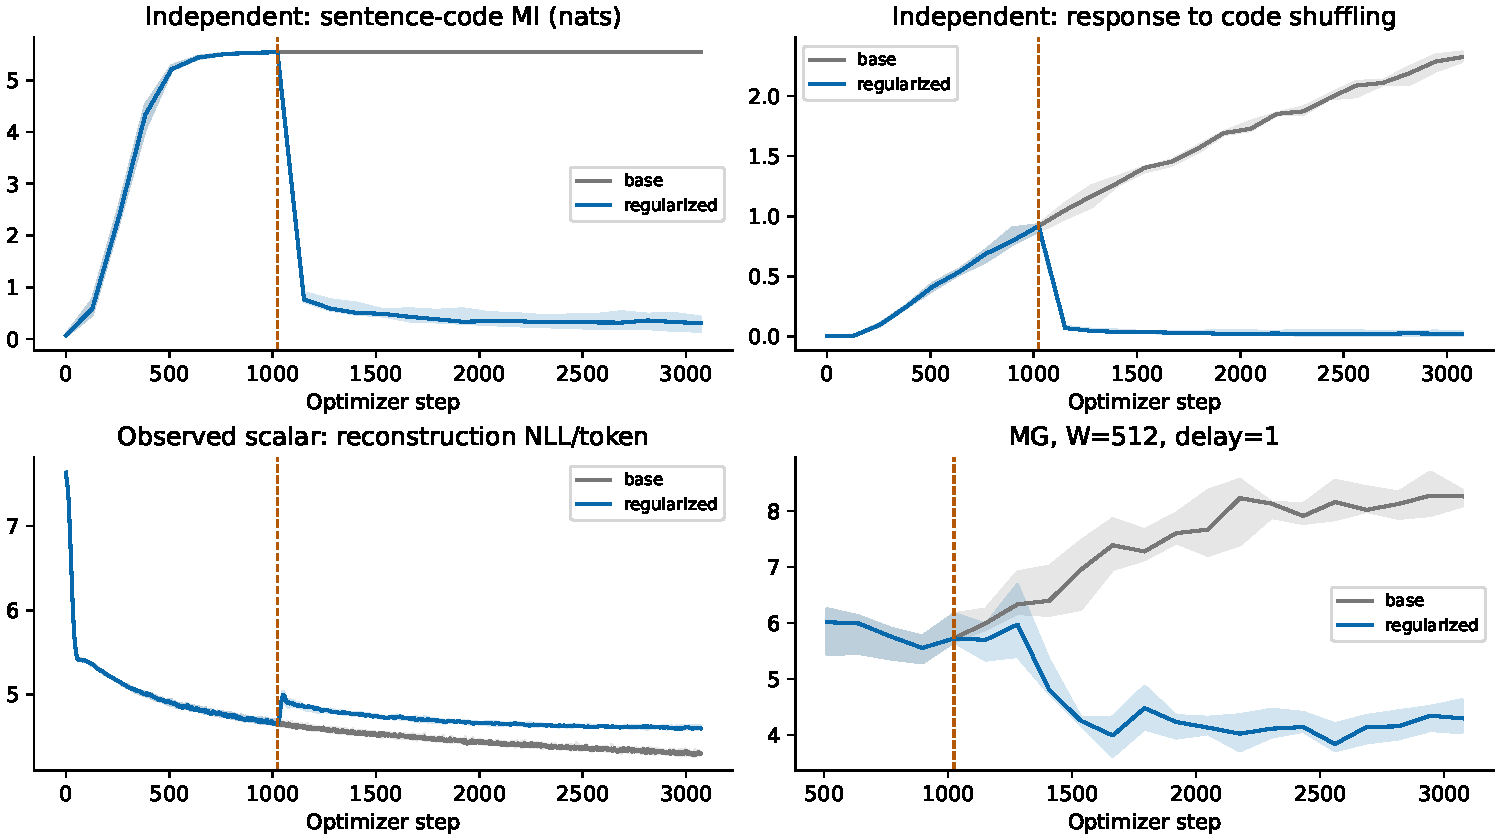
\includegraphics[width=\linewidth,height=.30\textheight,keepaspectratio]{expanded_figure.pdf}\end{center}

Линия --- медиана по seeds 1--9, полоса --- межквартильный диапазон, не доверительный интервал. Серый --- base, синий --- regularized; вертикаль --- развилка. Сверху независимые показатели, снизу входной скаляр и MG. На каждом шаге объединяются одни и те же девять seed; пилот не включён. Отдельные графики каждой пары сохранены.

\textbf{Оценка разброса:} медиана $q$ по девяти подтверждающим seed --- 0,517; 95\% percentile bootstrap-интервал медианы --- [0,480; 0,542], 20000 ресэмплирований пар seed. Для семи добавленных seed медиана --- 0,517. Интервал описывает вариацию инициализаций/батчей при фиксированных данных и probe; перенос на другие корпуса им не проверяется.

\newpage

\section*{4. Устойчивость, альтернативы и границы вывода}

\textbf{Дополнительный контроль сохранения кода:} критерий защиты выполнен в 9/9 продолжений; MG выше, чем при потере информации, в 9/9 из них (медиана отношения по всей девятке 1,286). Постановка и ограничения --- раздел 5.

\begin{center}\small
\begin{tabularx}{\linewidth}{>{\raggedright\arraybackslash}Xrr}
\toprule
Окно, delay & Медиана $q$ [минимум; максимум] & $q<1$, seeds 1--9 \\
\midrule
256, 1 & 0,499 [0,454; 0,553] & 9 / 9 \\
512, 1 & 0,517 [0,430; 0,599] & 9 / 9 \\
1024, 1 & 0,536 [0,452; 0,594] & 9 / 9 \\
512, 4 & 0,898 [0,707; 1,084] & 7 / 9 \\
\bottomrule\end{tabularx}\end{center}

Основной вариант --- 512, delay 1. Окно 1024 имеет только одно окно до перехода, поэтому это более слабая проверка. При delay 4 эффект может существенно ослабевать. Ни один вариант не заменял основной после просмотра результатов; полная таблица по каждому seed сохранена отдельно.

\begin{center}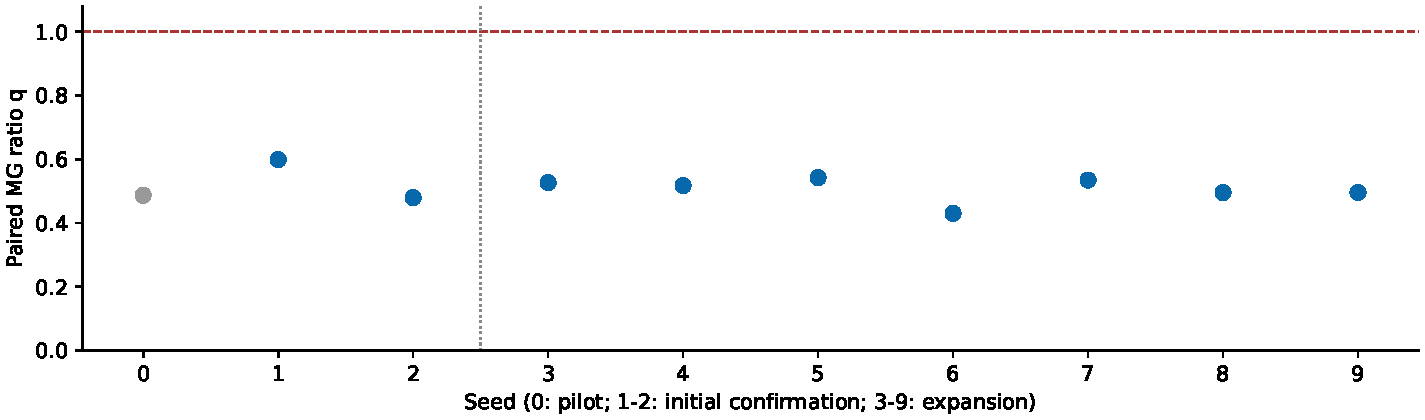
\includegraphics[width=\linewidth,height=.30\textheight,keepaspectratio]{seed_effects.pdf}\end{center}

Каждая точка --- одна парная инициализация. Seed 0 показан серым как пилот; пунктир после seed 2 отделяет семь добавленных запусков. Красная линия $q=1$ соответствует отсутствию дополнительного снижения относительно base.

\textbf{Наблюдатель важен.} Для обычного minibatch loss диапазон $q$ равен 0,973--1,028; $q<1$ в 4/9 случаев. Эти значения нельзя подменять результатом фиксированного probe. Для стандартного отклонения того же фиксированного loss медиана парного отношения --- 0,579, снижение относительно base в 9/9; для спектральной энтропии --- 0,645, в 9/9. Это дешёвые конкуренты, поэтому преимущество MG перед существующей диагностикой пока не установлено.

\textbf{Не абсолютная размерность.} В основном варианте у подтверждающих seed численно вырожденных окон: 0. Отношение оценок embedding 40/20: 0,97--2,03. Численная невырожденность сама по себе не подтверждает условия размерностной интерпретации. Рекуррентность здесь не установлена. Проверка масштаба x10 пройдена; IAAFT-суррогаты не дают основания приписывать сигналу доказанное восстановление особой нелинейной геометрии.

\textbf{Что подтверждено:} воспроизводимость сопутствующего сигнала MG при независимо измеренном ослаблении использования кода в данной NLP-постановке. \textbf{Что ещё не установлено:} универсальная специфичность детектора, преимущество перед KL и простыми статистиками, улучшение генеративного качества, другие корпуса и LLM. Reconstruction NLL не является marginal likelihood или perplexity генерации из prior: encoder видит восстанавливаемое предложение. Контроль с сохранением значительной части информации теперь выполнен; см. раздел 5.

Расчёты выполнены на CPU; часть запусков шла параллельно, поэтому времена этих запусков не используются для сравнительного benchmark. Дополнительный forward фиксированного probe имеет стоимость. Корпус и наблюдатель во всей серии одни и те же: десять seed расширяют проверку воспроизводимости, но не число независимых задач.

Источники постановки: Bowman et al., Generating Sentences from a Continuous Space, CoNLL 2016, K16-1002; He et al., Lagging Inference Networks and Posterior Collapse in Variational Autoencoders, ICLR 2019, arXiv 1901.05534. Все численные результаты получены нашими запусками. Исходный отчёт по трём seed сохранён в initial\_three; основной manuscript не менялся.


\newpage

\section*{5. Сохранение информации при том же внешнем коэффициенте KL}

\textbf{Зачем этот контроль.} В исходном сравнении менялись одновременно коэффициент регуляризации и использование кода. Добавлена третья ветвь к каждому сохранённому состоянию на шаге 1024: тот же переход beta с 0,01 на 1, но с защитой кода. Это продолжения прежних десяти инициализаций; основные числа ниже --- по seeds 1--9, пилот отдельно. Все ветви имеют одинаковые исходные веса, Adam, последовательность основных батчей и латентного шума.

\textbf{Выбор защиты без MG.} Пять дополнительных шагов encoder на пилоте не удержали код: информация упала с 5,48 до 0,52 нат. После этого применён заранее предусмотренный free bits: каждый средний по батчу KL отдельной координаты заменяется максимумом с 0,5 нат, затем значения суммируются по 16 координатам. Ниже порога штраф не создаёт градиента, подавляющего эту координату. Остальная процедура прежняя. Это изменение формы функции потерь, поэтому контроль не изолирует одну только величину beta.

Пилотная защита выбрана по независимым характеристикам, до расчёта её MG: поздняя информация и реакция на перестановку каждая должны сохранять не менее половины исходного уровня и превышать regularized минимум вдвое. Затем вариант зафиксирован для всех девяти остальных seed. Критерий выполнен в \textbf{9/9}; отбор по MG не проводился. Защита частичная, полного сохранения информации не предполагаем.

\begin{center}\small
\begin{tabularx}{\linewidth}{l>{\raggedright\arraybackslash}X>{\raggedright\arraybackslash}X>{\raggedright\arraybackslash}X>{\raggedright\arraybackslash}X}
\toprule
Ветвь & Информация, нат & Реакция на код & MG & MG / base \\
\midrule
Исходный контроль & 5,545 & 2,087 & 8,129 & 1,000 \\
Усиление KL & 0,327 & 0,021 & 4,172 & 0,517 \\
Усиление KL + free bits & 3,934 & 0,599 & 5,491 & 0,639 \\
\bottomrule\end{tabularx}\end{center}

Сначала берётся поздняя медиана внутри каждого seed, затем медиана по девяти seed. Последний столбец --- медиана парных отношений, не отношение медиан предыдущего столбца. Поздний интервал --- шаги 2048--3072; MG: окно 512, delay 1. Все индивидуальные тройки приведены в отдельном отчёте protection/report\_ru.pdf.

\begin{center}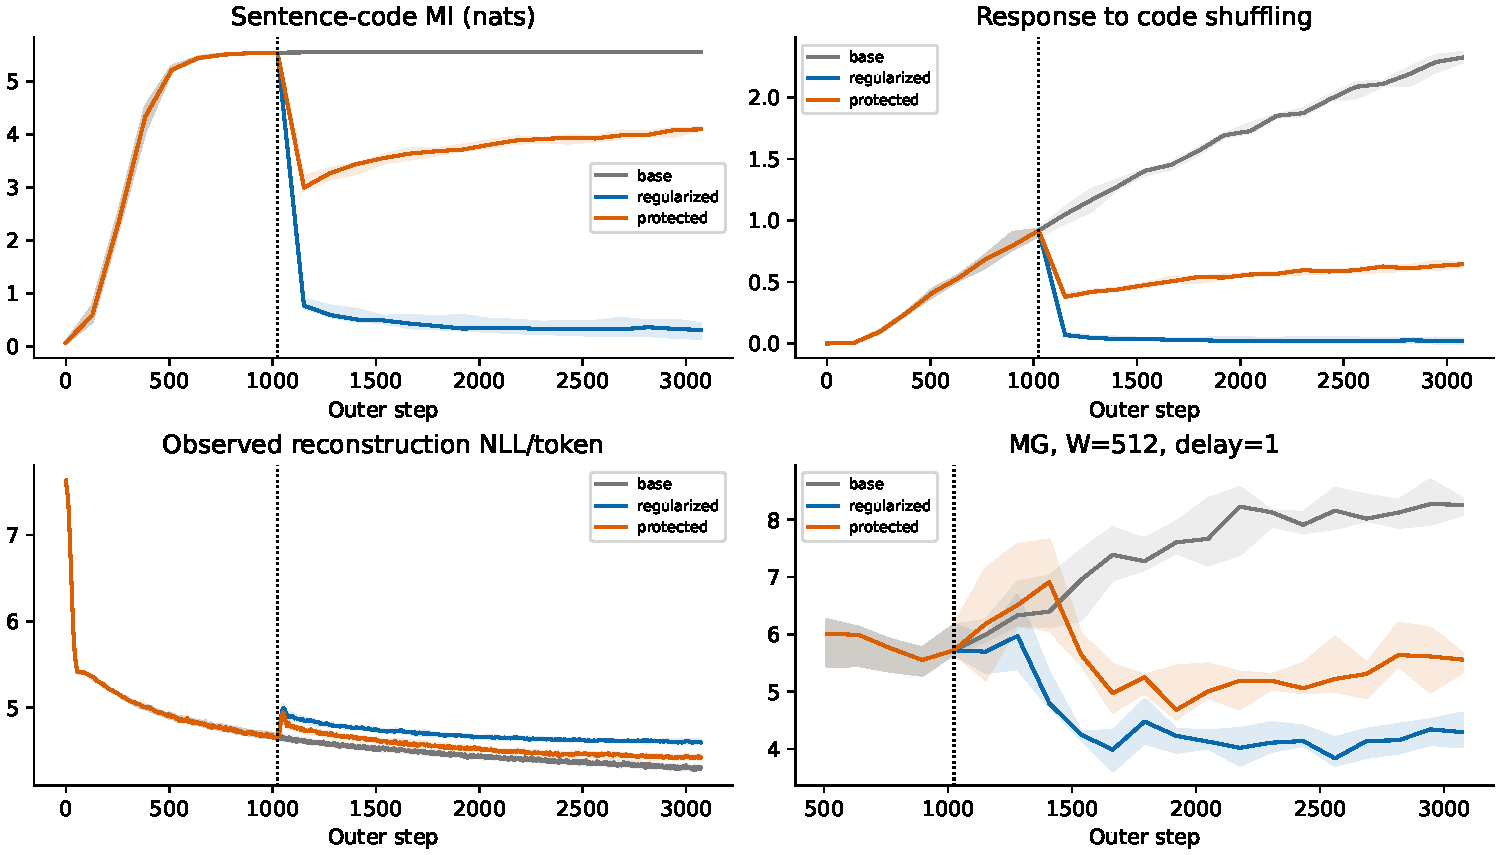
\includegraphics[width=\linewidth,height=.30\textheight,keepaspectratio]{protection/comparison_cohort.pdf}\end{center}

Медиана и межквартильный диапазон по seeds 1--9. Серый --- base, синий --- regularized, оранжевый --- free bits. Сверху независимые показатели использования кода, снизу входной reconstruction loss и MG.

\textbf{Результат.} Среди успешных защит MG выше regularized в 9/9 и ближе к base в 9/9. Медиана парного отношения protected/regularized по всей девятке --- 1,286; 95\% bootstrap-интервал медианы среди успешных защит --- [1,179; 1,418]. При этом медиана protected/base составляет 0,639, против 0,517 у regularized: защита не возвращает MG к исходному контролю.

\textbf{Как трактовать.} Различие MG согласуется с меньшей потерей информации в защищённой ветви в этой постановке. Это усиливает исходное наблюдение, но не доказывает, что любой спад MG означает потерю информации: информация сохранена лишь частично, а free bits меняет оптимизацию. Стандартное отклонение того же loss также выше при защите в 9/9: преимущество MG над простой статистикой не установлено. Дополнительные запуски не являются benchmark времени: они выполнялись параллельно.

Код, протокол до запусков, неудачная попытка encoder5, все десять защищённых ветвей и проверки сохранены в protection/. Предыдущая версия отчёта --- before\_protection/. Идея free bits: Kingma et al., Improved Variational Inference with Inverse Autoregressive Flow, NeurIPS 2016, Appendix C (arXiv 1606.04934).
\end{document}